\chapter{Result} \label{ch:result}
The INTERACTION Dataset \footnote{https://interaction-dataset.com/} is used to compare the algorithms and models of traffic participant tracking. The dataset contains multiple scenario in different locations where each scenario consists of multiple participants. Each participant is identified by an id for each scenario and each frame per 0.1s has a set of vehicles and their position. The x and y position of the vehicle is noted per time step and the algorithms aforementioned are applied to compare. The initial state of the system is set using the table \ref{eq:initial}
\begin{equation*}
\label{eq:initial}
\begin{split}
x_0 &= zonotope([zeros(n), diag([1000;1000;10;10;10;10])])\\
w_k &= [0.1;0.1;0.4;0.4;0.1;0.1]\\
v_k &= [0.1;0.1]
\end{split}
\end{equation*}

\begin{figure}
\begin{subfigure}{.5\textwidth}
\centering
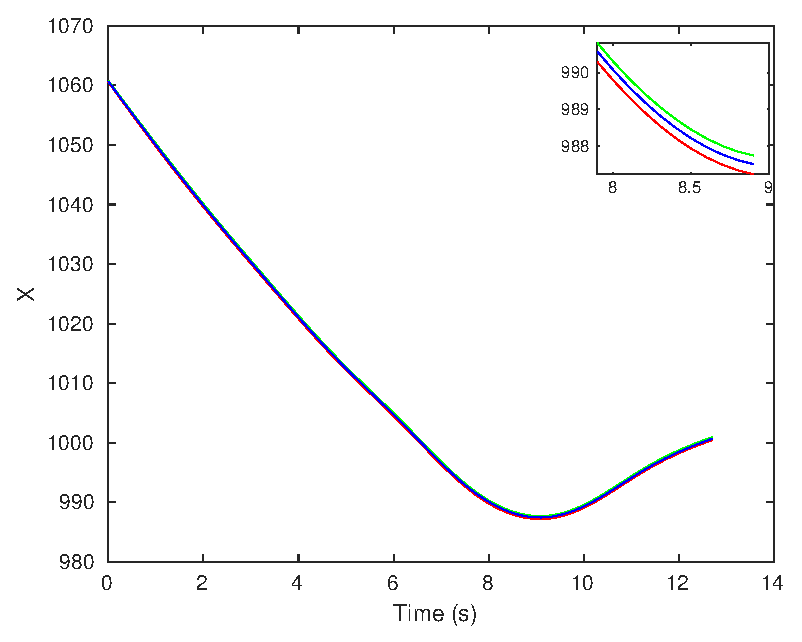
\includegraphics[width=.8\linewidth]{figures/s_caXzoomed}
\caption{Estimating $x$}
\end{subfigure}
\begin{subfigure}{.5\textwidth}
\centering
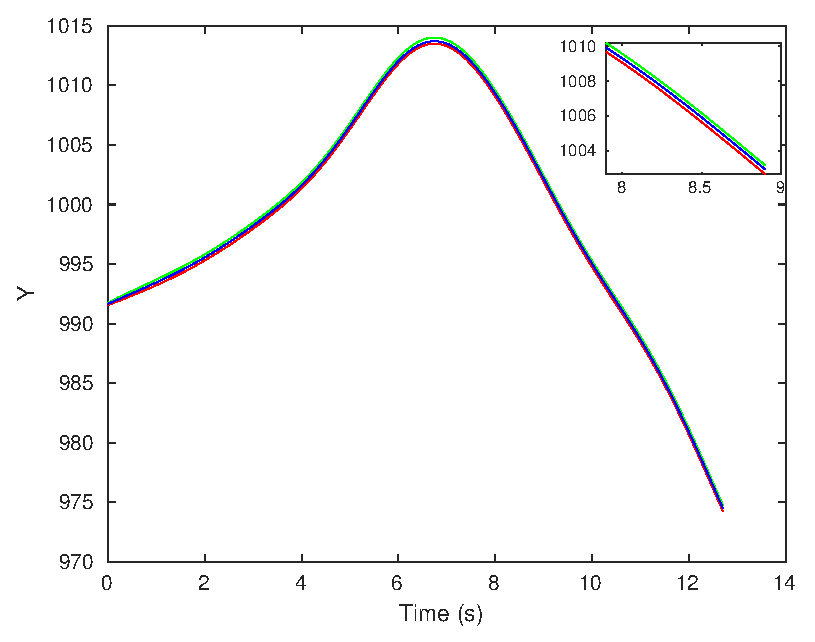
\includegraphics[width=.8\linewidth]{figures/s_caYzoomed}
\caption{Estimating $y$}
\end{subfigure}
\begin{subfigure}{.5\textwidth}
\centering
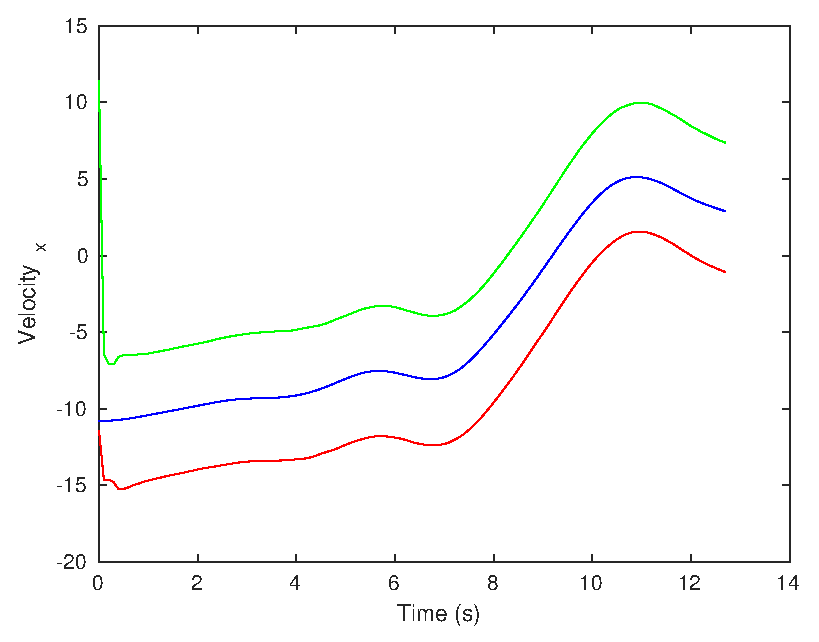
\includegraphics[width=.8\linewidth]{figures/s_caVelocity_x}
\caption{Estimating $velocity_x$}
\end{subfigure}
\begin{subfigure}{.5\textwidth}
\centering
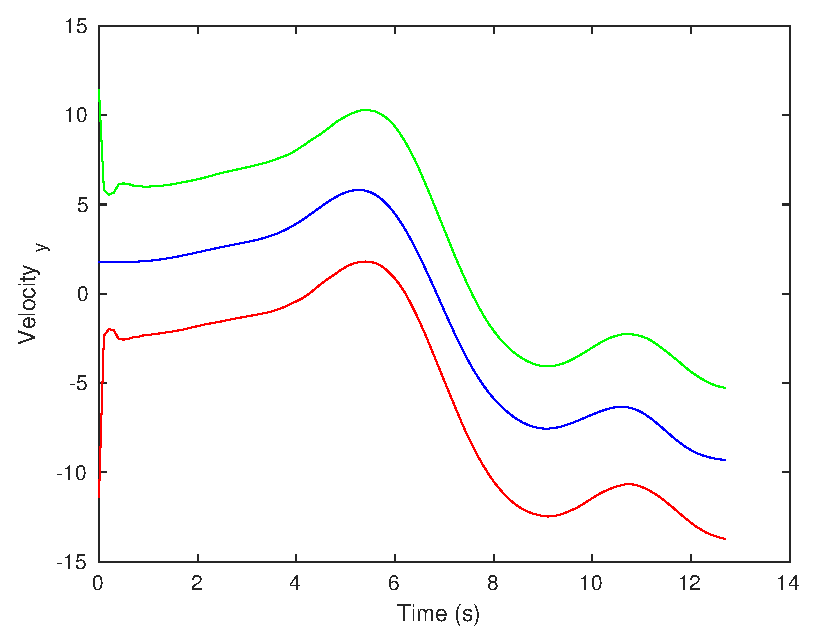
\includegraphics[width=.8\linewidth]{figures/s_caVelocity_y}
\caption{Estimating $velocity_y$}
\end{subfigure}
{\color{red}\rule{.1\linewidth}{1pt}} : Lower bound of estimation\\
{\color{green}\rule{.1\linewidth}{1pt}} : Upper bound of estimation\\
{\color{blue}\rule{.1\linewidth}{1pt}} : True value
\caption{Segment Minimization using Frobenius norm}
\end{figure}


\begin{figure}
\begin{subfigure}{.5\textwidth}
\centering
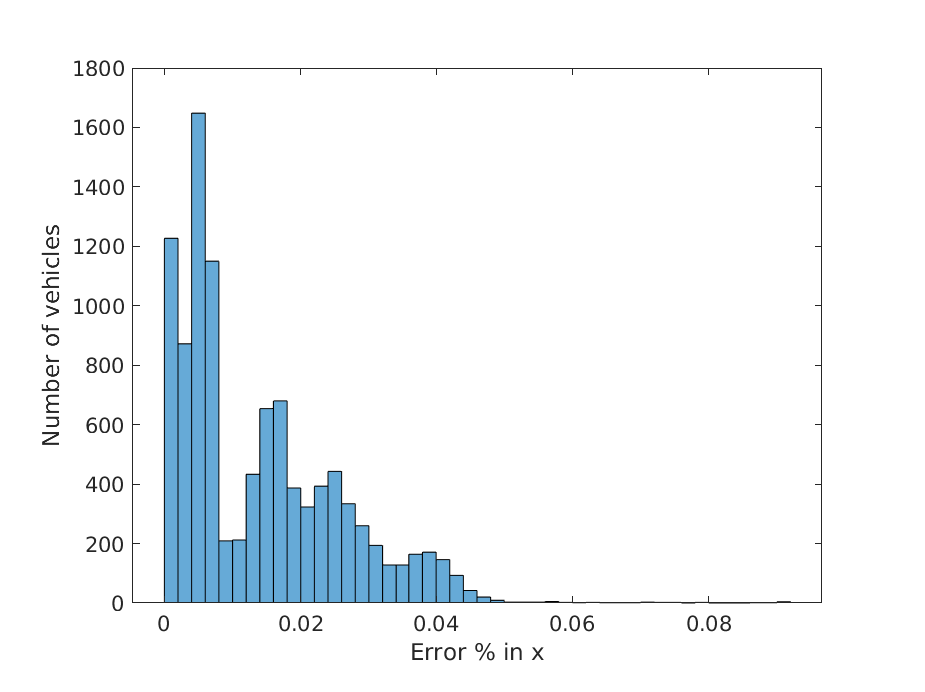
\includegraphics[width=.8\linewidth]{figures/s_caXerror}
\caption{RMSE $x$}
\end{subfigure}
\begin{subfigure}{.5\textwidth}
\centering
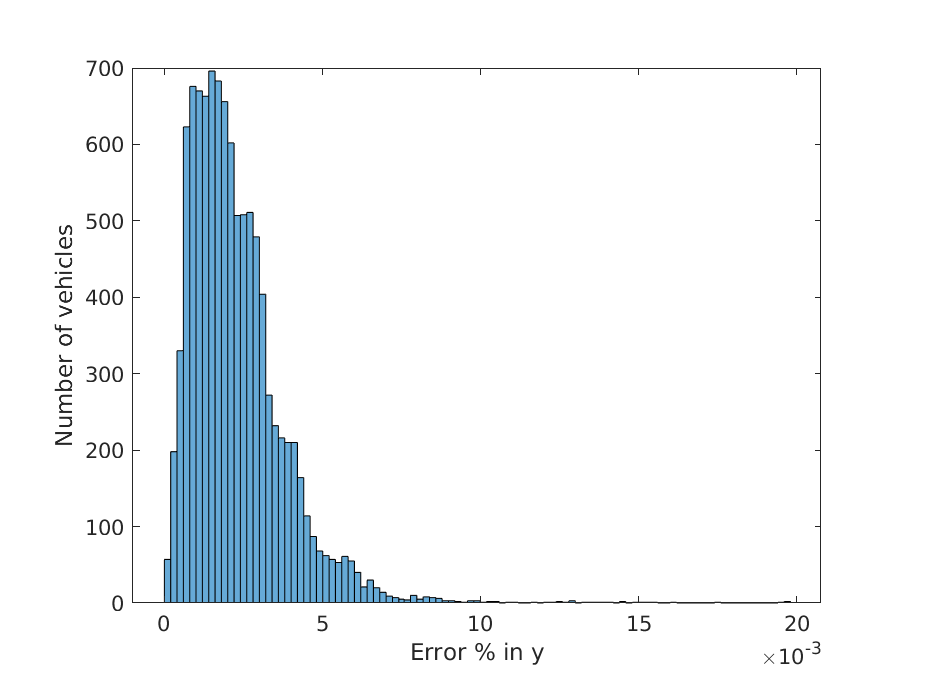
\includegraphics[width=.8\linewidth]{figures/s_caYerror}
\caption{RMSE $y$}
\end{subfigure}
\begin{subfigure}{.5\textwidth}
\centering
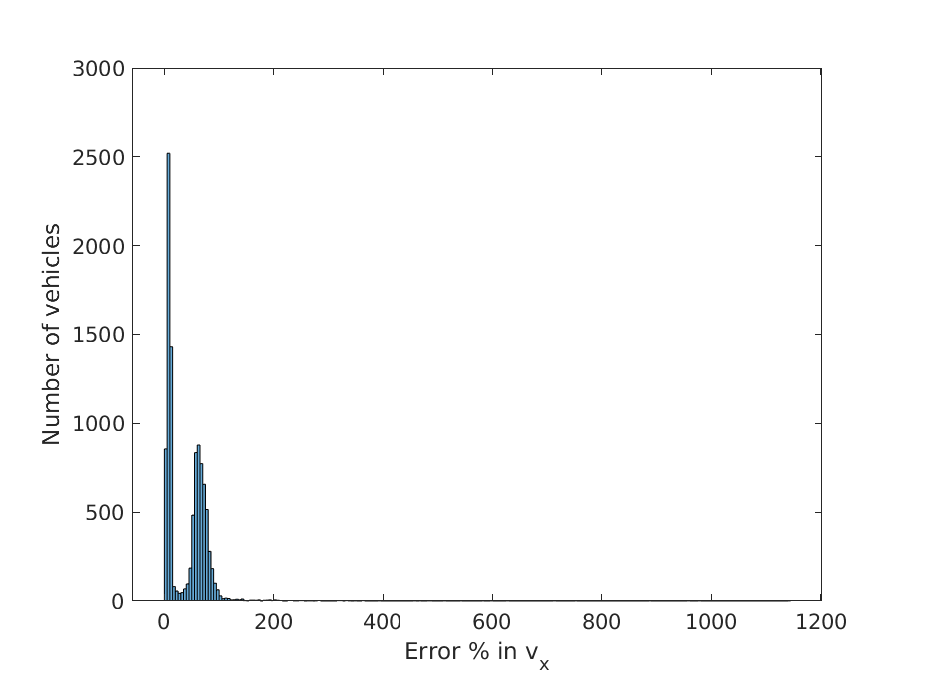
\includegraphics[width=.8\linewidth]{figures/s_cavXerror}
\caption{RMSE in $velocity_x$}
\end{subfigure}
\begin{subfigure}{.5\textwidth}
\centering
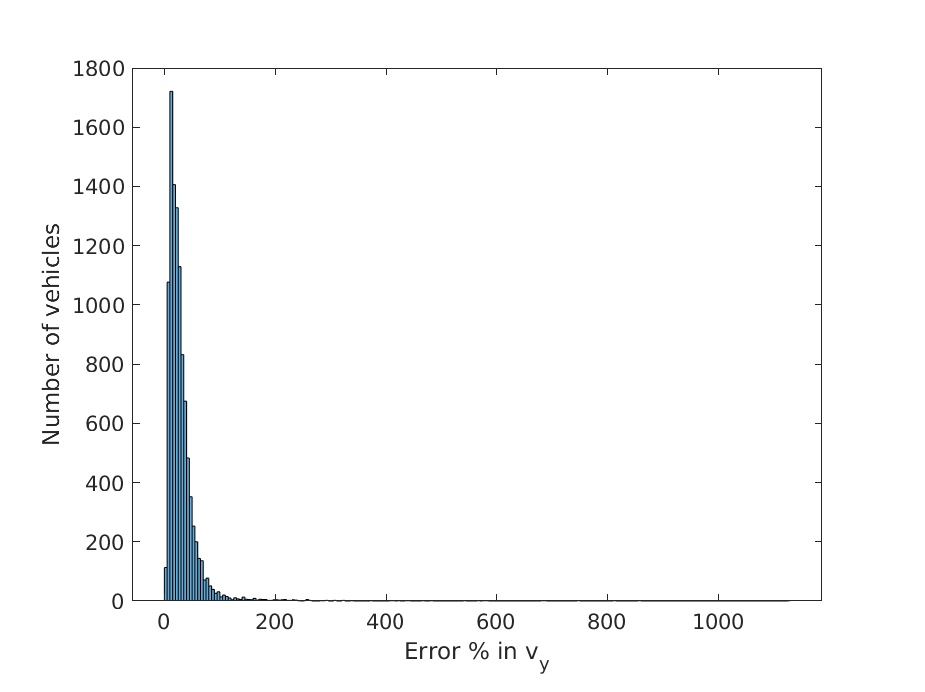
\includegraphics[width=.8\linewidth]{figures/s_cavYerror}
\caption{RMSE in $velocity_y$}
\end{subfigure}
\caption{Histogram of errors from Segment Minimizer on 651 vehicles }
\end{figure}
%\begin{itemize}
%\item{Efficiency}
%\item{Accuracy}
%\item{Performance Metric}
